\def\myscale{0.3}
\def\greythick{50}

\begin{subfigure}{0.45\textwidth}
\centering
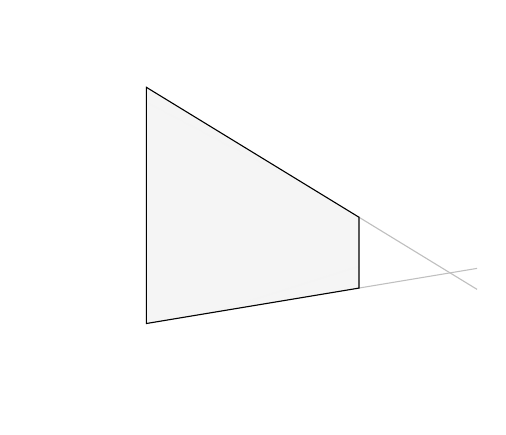
\begin{tikzpicture}[scale=\myscale]
	\coordinate(TL) at (1,6.5);
	\coordinate(BL) at (1,-3.5);
	\coordinate(TR) at (10,1);
	\coordinate(BR) at (10,-2);
	
	% Draw some white lines to make sure all figures are the same size:
	\draw[white] (-4,8.5) -- (15,-1.5);
	\draw[white] (-4,-5.5) -- (15,0.5);
	\draw[white] (1,-7) -- (1,9);
	\draw[white] (11,-7) -- (11,9);
	
	% Draw the singular regions:
	\draw[gray!\greythick] (10,1) -- (15,-2.05555556);
	\draw[gray!\greythick] (10,-2) -- (15,-1.16666667);
	
	% Draw the trapezium:
	\filldraw[fill=black!5, fill opacity=0.8] (BL) -- (BR) -- (TR) -- (TL) -- cycle;
\end{tikzpicture}
\caption{}\label{fig:p2singularitiesa}
\end{subfigure}
\begin{subfigure}{0.45\textwidth}
\centering
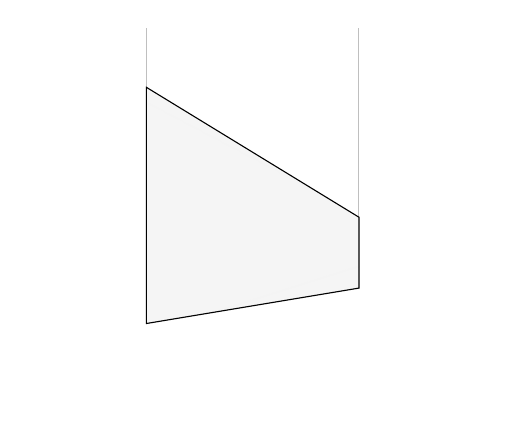
\begin{tikzpicture}[scale=\myscale]
    \coordinate(TL) at (1,6.5);
    \coordinate(BL) at (1,-3.5);
    \coordinate(TR) at (10,1);
    \coordinate(BR) at (10,-2);
	
	% Draw some white lines to make sure all figures are the same size:
	\draw[white] (-4,8.5) -- (15,-1.5);
	\draw[white] (-4,-5.5) -- (15,0.5);
	\draw[white] (1,-7) -- (1,9);
	\draw[white] (11,-7) -- (11,9);
	
	% Draw the singular regions:
	\draw[gray!\greythick] (1,6.5) -- (1,9);
	\draw[gray!\greythick] (10,1) -- (10,9);
	
	% Draw the trapezium:
	\filldraw[fill=black!5, fill opacity=0.8] (BL) -- (BR) -- (TR) -- (TL) -- cycle;
\end{tikzpicture}
\caption{}\label{fig:p2singularitiesb}
\end{subfigure}
\begin{subfigure}{0.45\textwidth}
    \centering
    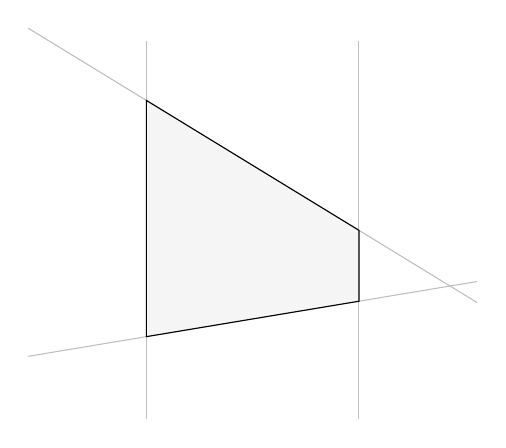
\begin{tikzpicture}[scale=\myscale]
    \coordinate(TL) at (1,6.5);
    \coordinate(BL) at (1,-3.5);
    \coordinate(TR) at (10,1);
    \coordinate(BR) at (10,-2);
	
	% Draw the singular regions:
	\draw[gray!\greythick] (-4,9.55555556) -- (15,-2.05555556);
	\draw[gray!\greythick] (-4,-4.33333333) -- (15,-1.16666667);
	\draw[gray!\greythick] (1,-7) -- (1,9);
	\draw[gray!\greythick] (10,-7) -- (10,9);
	
	% Draw the trapezium:
	\filldraw[fill=black!5, fill opacity=0.8] (BL) -- (BR) -- (TR) -- (TL) -- cycle;
\end{tikzpicture}
\caption{}\label{fig:p2singularitiesc}
\end{subfigure}

